\section{Day 22: Lifting, Fundamental Group of Circle; Categories (Nov. 21, 2024)}
Outfit of the day: homeland defender sniper monkey palette
\begin{figure}[h]
    \centering
    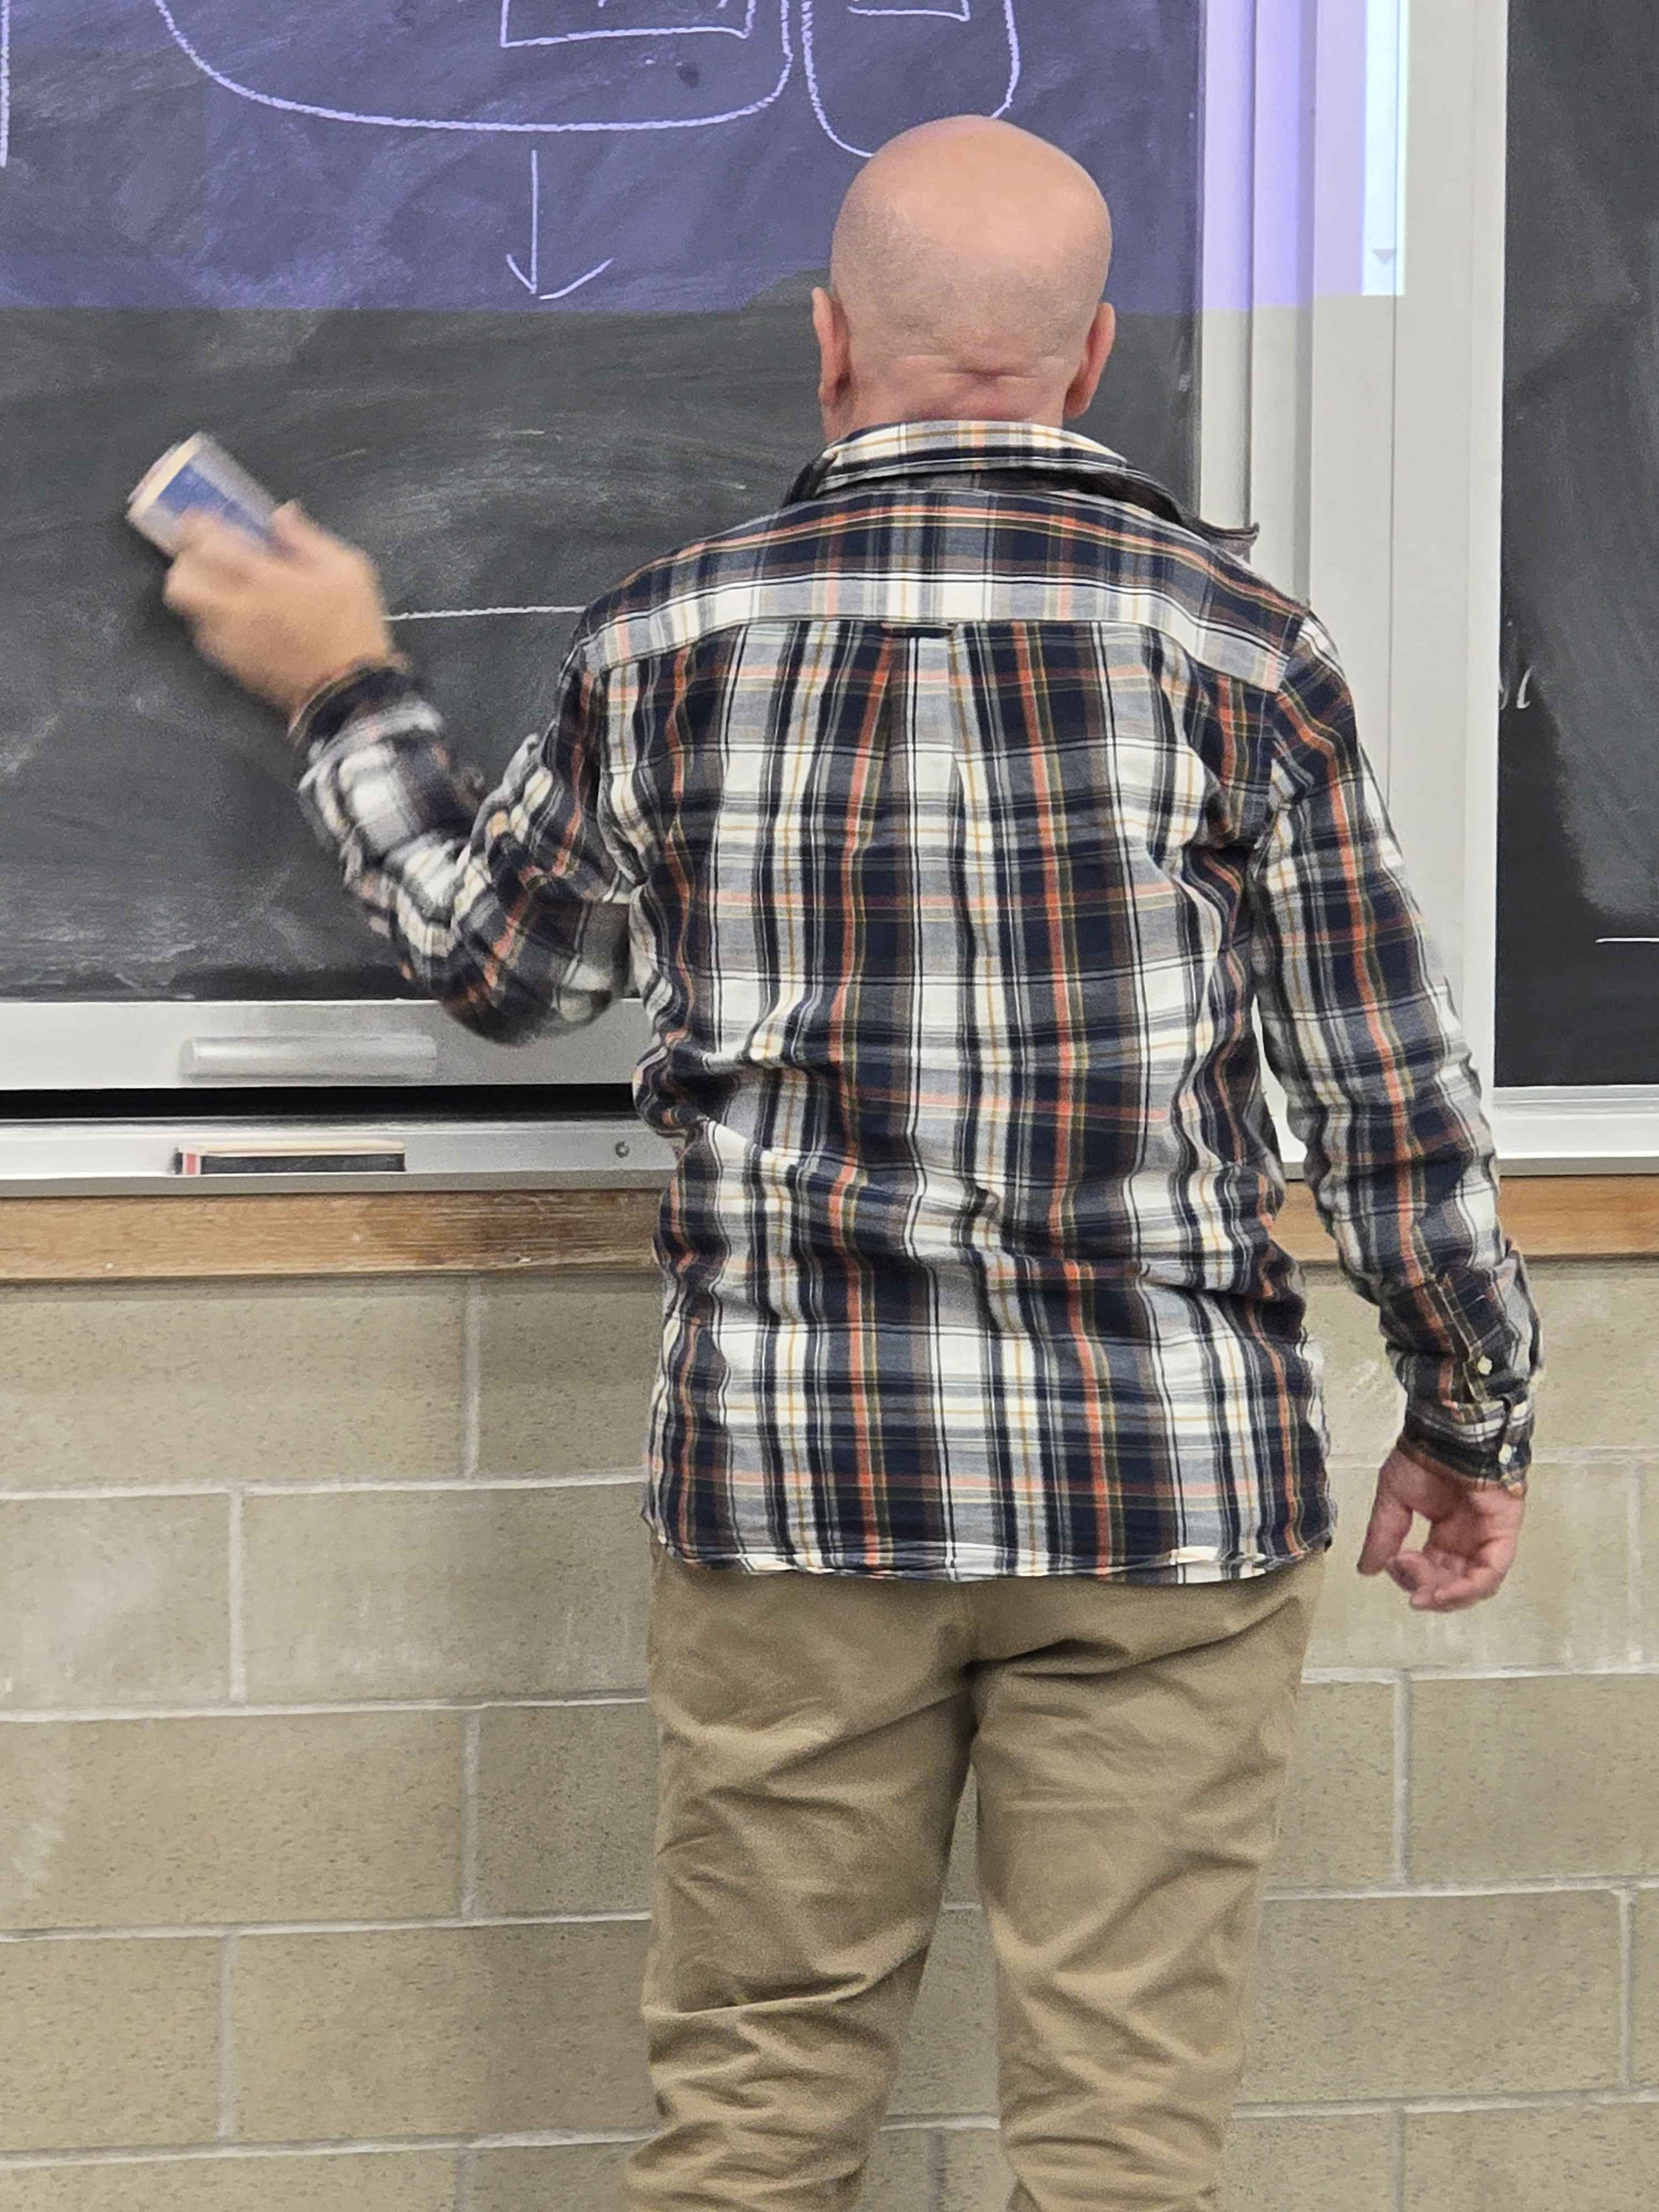
\includegraphics[scale=0.1]{MAT327 Notes/Dror Shirts/dror day 22 shirt.jpg}
\end{figure}

\noindent Recall the path/homotopy lifting property: Given a covering $p : (E, e_0) \to (B, b_0)$ and $\gamma : (I, 0) \to B, b_0)$ or $H : (I^2, 0) \to (b, b_0)$, there exists a unique lift $\tilde{\gamma} : (I, 0) \to (E, e_0)$ or $\tilde{H} : (I^2, 0) \to (E, e_0)$ such that $p \circ \tilde{\gamma} = \gamma$ and $p \circ \tilde{H} = H$.
\begin{simplethm}
    $\pi_1(s^1, 1) \cong \ZZ$.
\end{simplethm}
\noindent For the purpose of the proof, fix $(E, e_0) = (\RR, 0)$, and $(B, b_0) = (S^1, 1)$, and $p : (E, e_0) \to (B, b_0)$ is just the complex exponential map, $p(x) = e^{2\pi i x}$.
\medskip\newline
\noindent For $n \in \ZZ$, $s \in I$, let $\varphi(n)(s)$ be a homotopy class of a path, given by
\[ \varphi(n)(s) = p(ns) = e^{2 \pi i n s}. \]
Here, $\gamma : [0, 1] \to S^1$, $\gamma(0) = \gamma(1) = 1$, and we have that $\psi([\gamma]) = \tilde{\gamma}(1)$, where $\tilde{\gamma}$ is the lift of $\gamma$ as in the proof above. We also have that $\tilde{\gamma}(0) = 0$. Note that $p(\tilde{\gamma}(1)) = \gamma(1) = 1$, since $[\gamma] \in \pi_1(S^1, 1)$. Thus, $\tilde{\gamma}(1) \in p^{-1}(1) = \ZZ$. We need to show:

\newpage
\begin{enumerate}[label=(\alph*)]
    \item $\psi$ is well-defined.
    \item $\psi \circ \varphi = \id_{\ZZ}$.
    \item $\varphi \circ \psi : \id_{\pi_1}$.
    \item $\varphi$, $\psi$ are group homomorphisms if and only if $[\varphi(n + m)] = [\varphi(n)] \ast [\varphi(m)]$.
\end{enumerate}
We prove the claims now.
\begin{enumerate}[label=(\alph*)]
    \item If $\gamma_1 \sim_p \gamma_2$ and $\gamma_1(0) = \gamma_2(0) = \gamma_1(1) = \gamma_2(1) = 1$, then we need to show that $\tilde{\gamma_1}(1) = \psi([\gamma_1]) = \psi([\gamma_2]) = \tilde{\gamma_2}(1)$. We know that there exists $H : I^2 \to (B, b_0)$ such that $H(s, 0) = \gamma_1(s), H(s, 1) = \gamma_2(s)$, and $H(0, t) = H(1, t) = 1$. Let $\tilde{H}$ be the lift of $H$.
    \medskip\newline
    We know $\tilde{H}(0, 0) = 0$, and $p(\tilde{H}(s, 0)) = H(s, 0) = \gamma_1(s)$, and so $\tilde{H}(s, 0)$ is a lift of $\gamma_1$. In particular, $\tilde{H}(s, 0) = \tilde{\gamma_1}(s)$ by uniqueness in the theorem above. Similarly, $\tilde{H}(0, t) = 0$. In particular, $\tilde{H}(0, 1) = 0$; this means we have that $\tilde{H}(s, 1) = \tilde{\gamma_2}(s)$. Now, use the path lifting theorem but with $p : (\RR, \tilde{\gamma}(1)) \to (S^1, 1)$. By uniqueness of path lifting, $\tilde{H}(1, t)$ is the constant $\tilde{\gamma_1}(1)$, and so $\tilde{\gamma_2}(t) = \tilde{H}(1, 1) = \tilde{\gamma_1}(1)$. \qed

    \item Given $n$, $\varphi(n) = [\gamma_n]$, where $\gamma_n(s) = p(ns)$. Let $\tilde{\gamma_n}$ be the lift of $\gamma_n$; then $\tilde{\gamma_n}(s) = ns$. So $\psi(\varphi(n)) = \tilde{\gamma_n}(1) = n \cdot 1 = n$. \qed
    
    \item Let $[\gamma] \in \pi_1(S^1, 1)$. Let $\tilde{\gamma}$ be a lift of $\gamma$, $\tilde{\gamma} : [0, 1] \to \RR$, such that $p(\tilde{\gamma}(s)) = \gamma(s)$. Let $n = \tilde{\gamma}(1)$, and then $\varphi(n) = \gamma_n$. We need to show that $\gamma \sim_p \gamma_n$. Note that $\tilde{\gamma}(0) = 0$, $\tilde(\gamma_n)(0) = 0$; $\tilde{\gamma}(1) = n$, $\tilde{\gamma_n}(1) = n$, $\tilde{\gamma_n}(s) = ns$. So there exists a homotopy $\overline{H}$ in $\RR$ from $\tilde{\gamma}$ to $\tilde{\gamma_n}$ with endpoints $0$ to $n$. Let $H = p \circ \overline{H}$; then we have a homotopy $\gamma \sim_p \gamma_n$.
    
    \item We only sketch the proof for this one. $\varphi(n + m) = p(s \mapsto (n + m)s)$. Think of the expression as projecting the straight line given by $s \mapsto (n + m)s$. Then $\phi(n) \ast \phi(m)$ is intuitively a concatenation of $p$ on $s \mapsto ns$ and $s \mapsto ms$.
\end{enumerate}

\noindent We now introduce categories. We start by giving a few examples for intuition. Colloquially, categories consist of objects, morphisms, and morphism composition.
\begin{enumerate}[label=(\alph*)]
    \item Maps between vector spaces as objects, i.e. the morphisms are linear transformations and compositions, are a category. Topological spaces equipped with continuous functions and composition is also a category. Groups, homomorphisms, and compositions is also a category. Sets, functions, and compositions are also a category. Respectively, these are from MAT240, 327, 347, and 407.
\end{enumerate}
\begin{definition}
    A \textit{category} $\SC$ is a quadruple $(\mathrm{obj}_\SC, \mathrm{mor}_\SC, \circ, \id_\SC)$, where:
    \begin{itemize}
        \item objects are a collection, i.e. ``possibly a huge set'',
        \item for any two objects $A, B \in \mathrm{obj}_\SC$, we have a set $\mathrm{mor}_\SC(A, B)$.
        \item for any three objects $A, B, C \in \mathrm{obj}_\SC$, we have a function $\circ_{\SC, A, B, C} = \circ : \mathrm{mor}(A, B) \times \mathrm{mor}(B, C) \to \mathrm{mor}(A, C)$, where $(f, g) \mapsto g \circ f = \circ_{\SC, A, B, C}(f, g)$, for all $f \in \mathrm{mor}(A, B)$ and $g \in \mathrm{mor}(B, C)$.
        \item For each object, $A \in \mathrm{obj}$, a morphism $\id_A \in \mathrm{mor}(A, A)$, such that
        \begin{enumerate}[label=(\roman*)]
            \item Associativity; for all $A, B, C, D \in \mathrm{obj}$ and $f \in \mathrm{mor}(A, B)$, $g \in \mathrm{mor}(B, C)$, $h \in \mathrm{mor}(C, D)$, we have $h \circ (g \circ f) = (h \circ g) \circ f$.
            \item Given $A, B \in \mathrm{obj}$, $f \in \mathrm{mor}(A, B)$, we have $f \circ \id = \id \circ f = f$.
        \end{enumerate}
    \end{itemize}
\end{definition}
\noindent We now continue our examples.
\begin{enumerate}[label=(\alph*)]
    \setcounter{enumi}{1}
    \item Based topological spaces, where the objects are given by $\{(X, x_0)\}$, morphisms given by functions $(X, x_0)$ to $(Y, y_0)$, and path composition $\ast$.
    \item Let $\mathrm{obj} = X$, $\mathrm{mor}(x, y)$ be the set of equivalence classes of paths starting at $x$ and ending at $y$ where $x, y \in \mathrm{obj} = X$, composition given by $\ast$, and $\mathrm{id}$ given by the constant path $e_x$.
\end{enumerate}
A category in which all morphisms are invertible, i.e.
\[ f \in \mathrm{mor}(A, B) \implies \exists f^{-1} \in \mathrm{mor}(B, A) \]
is called a groupoid. In particular, (c) is an example of a groupoid.
\begin{enumerate}[label=(\alph*)]
    \setcounter{enumi}{3}
    \item The fifteen puzzle! The objects are given by the set of sixteen elements, of which the elements are where the empty square is placed. The morphisms between two fifteen puzzle positions are given by the ways to shuffle the tiles around; in particular, there are $15!$ shuffles (? proof?).
\end{enumerate}
